\documentclass[tikz,border=12pt]{standalone}
\usepackage{stix}
\usepackage{tikz}
\usetikzlibrary{angles}
\usetikzlibrary{quotes}
\usepackage{tkz-euclide}
\usetkzobj{all}
\usetikzlibrary{arrows, arrows.meta}
\definecolor{blue}{RGB}{0,51,255}
\definecolor{green}{RGB}{0,153,0}
\begin{document}
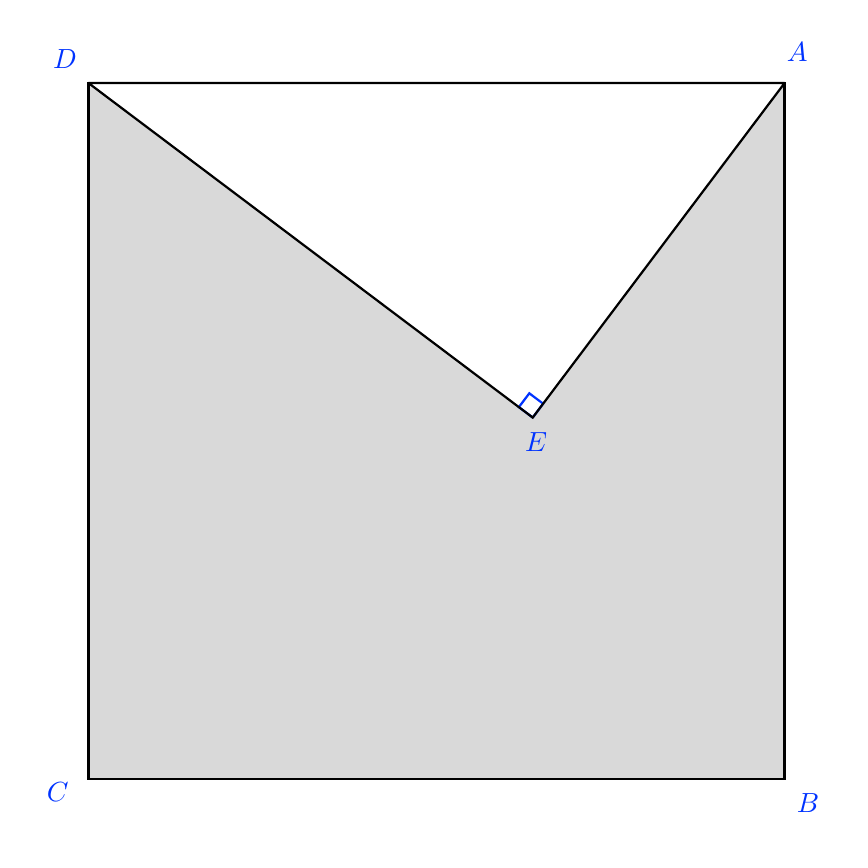
\begin{tikzpicture}
\pgfgettransformentries{\mya}{\myb}{\myc}{\myd}{\mys}{\myt}
\pgfmathsetmacro{\preserve}{1/\mya}
\begin{scope}[>={Stealth[scale=1.2]} , thick,rotate=0 ] 

\coordinate (A) at (0,0);
\coordinate (D) at (180 :8.8414);

\coordinate (x) at (180+ 53.021 : 0.5);
\path (D)--++ ( -36.979 : 0.5 ) coordinate (y);

\coordinate (E) at ( intersection of A--x and D--y);

\path (A)--(D)--([turn] 90:8.8414) coordinate(C);
\path (D)--(A)--([turn] -90:8.8414) coordinate(B);

\tkzMarkRightAngle[size=0.22*\preserve, color=blue,thick](A,E,D);

\path pic ["$A$", blue, angle radius=20]  {angle = B--A--C};
\path pic ["$B$", blue, angle radius=20]  {angle = C--B--A};
\path pic ["$C$", blue, angle radius=20]  {angle = A--C--B};
\path pic ["$D$", blue, angle radius=20]  {angle = A--D--C};
\path pic ["$E$", blue, angle radius=15]  {angle = D--E--A};

\draw [fill=gray!30] (A)--(B)--(C)--(D)--cycle;
\path pic ["$E$", blue, angle radius=15]  {angle = D--E--A};

\path [fill=white](A)--(E)--(D);
\tkzMarkRightAngle[size=0.22*\preserve, color=blue,thick](A,E,D);
\draw (A)--(E)--(D) (A)--(D);

\end{scope}
\end{tikzpicture}
\end{document}